\documentclass{article}
\usepackage{pdfpages}
\begin{document}
\section{Problem Statement}
2015 marked a record year for Americans that exercised regularly, hitting just about 55\%. However, keeping that momentum is difficult. As blue-collar jobs continue to decline, it has been more important than ever to keep a weekly regiment of eating healthy and exercising.

Living in the most inter-connected generation poses quite a viable idea for social networking: healthy living. With our knowledge of a database systems, we can build a social network that connects users to friends, peers and family to make an online community of healthy living.

Our database will be essential because it will unite something so mundane and uninteresting with people that are familiar, quite possibly making exercise fun and enjoyable. Maybe we can shape an entire generation by just having motivation a click away.

\section{Conceptual Database Design}
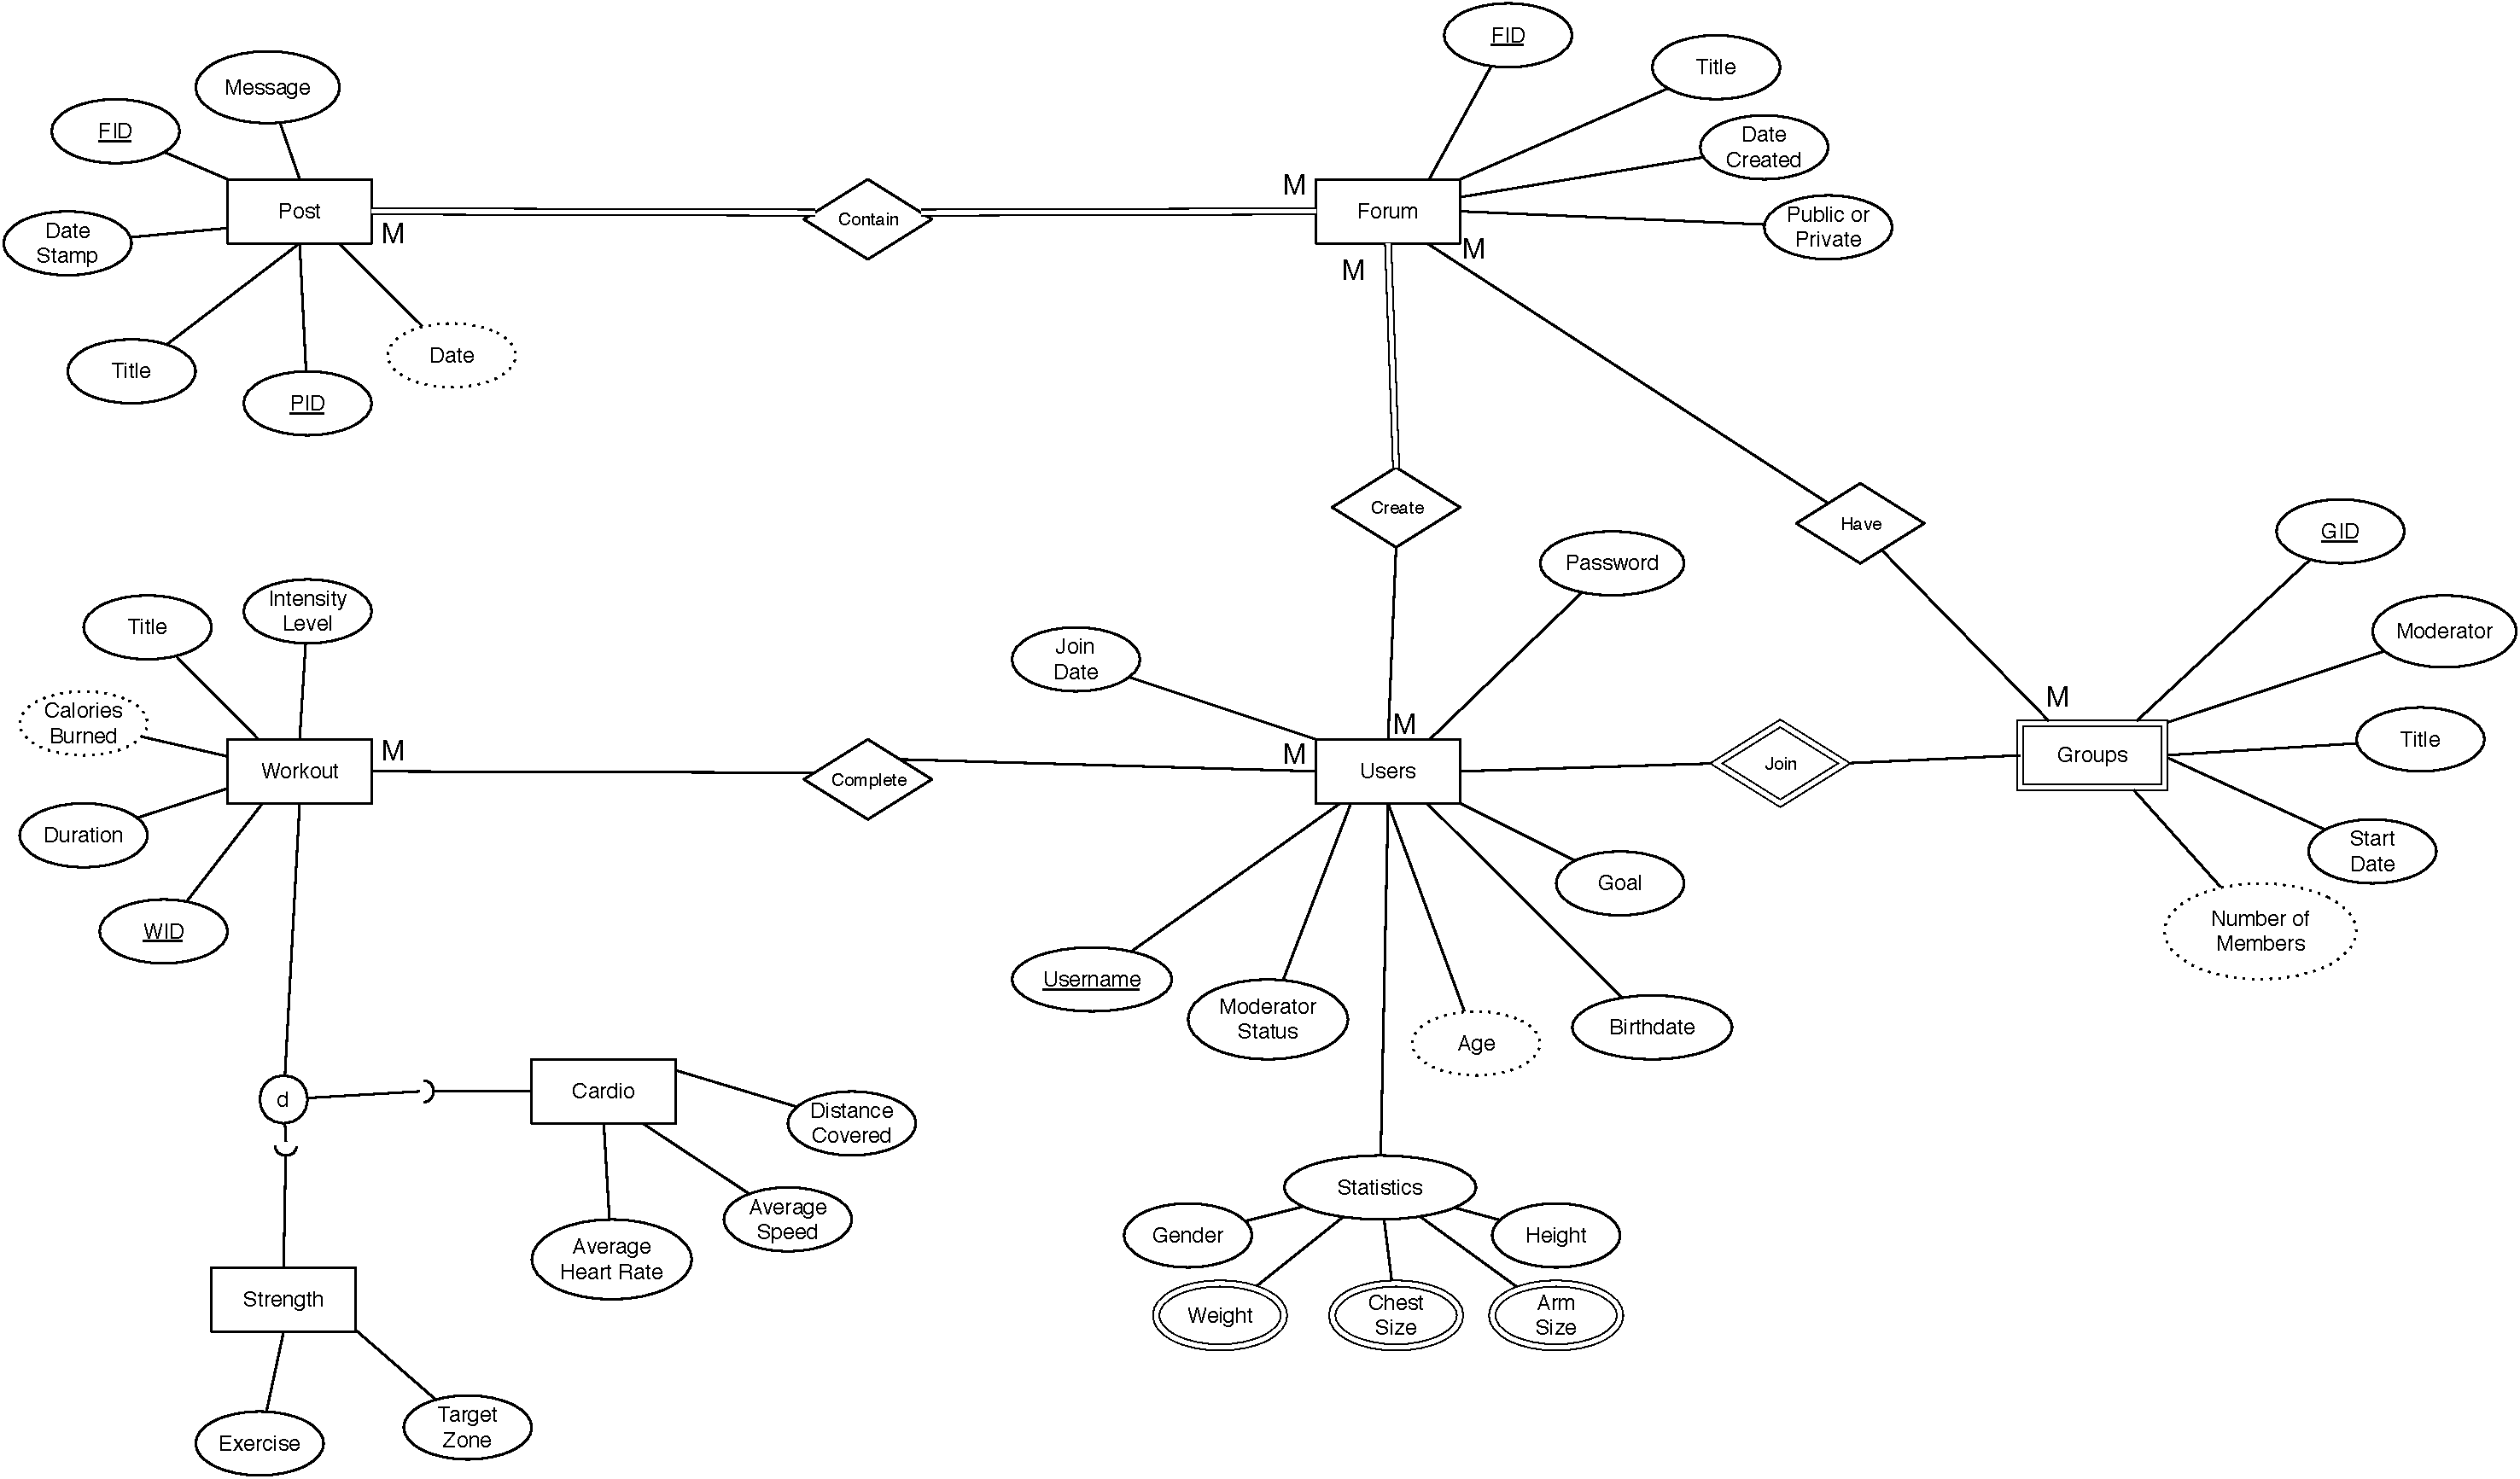
\includepdf[pages=-,width=1.75\textwidth]{ERR.pdf}

\section{Functional Requirement}
\begin{itemize}
    \item \textbf{Users} communicate with \textbf{users} by posting \textbf{posts}, using \textbf{forums}, etc.
    \item \textbf{Groups} contain \textbf{users} who communicate with each other.
    \item \textbf{Forums} contain posts.
    \item \textbf{Exercises} get queried by users.
    \item \textbf{Users} get queried by other \textbf{users.}
\end{itemize}


\end{document}